\documentclass[11pt]{article}
\usepackage[margin=1in]{geometry}
\usepackage{graphicx}
\usepackage{booktabs}
\usepackage{float}
\usepackage{amsmath}
\usepackage{xcolor}
\usepackage[hidelinks]{hyperref}
\usepackage{tikz}
\usetikzlibrary{shapes.geometric,arrows.meta,positioning,calc}
\graphicspath{{figures/}}

\tikzset{
  dfbox/.style ={rectangle, rounded corners=3pt, draw=black!65, thick,
                 fill=blue!8, minimum height=12mm, text width=20mm,
                 align=center, font=\small},
  dfsrc/.style ={dfbox, fill=black!8},
  flow/.style  ={-{Stealth[length=2mm,width=1.6mm]}, thick, draw=black!70}
}

\title{\textbf{Pro Team Multimodel --- In a Nutshell}\\[2pt]
\large A Short Guide to the Interactive Form S-6 Grid, Wind Fields,
Sensitivity, and Loss}
\author{Pro Team and Claude Code}
\date{\today}

\begin{document}
\maketitle

\begin{abstract}
\noindent This is the quick read. The \textbf{Pro Team Multimodel} is a zero-backend
web application that draws the official Form S-6 $21\times40$ grid over southern
Florida, runs three hurricane wind-field models over it, turns wind into loss through
a damage curve and an exposure book, and reports sensitivity, uncertainty, and loss
metrics---the five catastrophe-model disciplines (\emph{meteorology}, \emph{vulnerability},
\emph{statistics}, \emph{actuarial science}, \emph{computer science}) each made
swappable or explorable. The full derivations, validations, and references are in the
companion report; this document gives the essentials in one sitting. The single most
important finding: once the storm population is sampled realistically---one lumped set
of 200 storms carrying the observed dependence between hurricane parameters, rather than
stratified into intensity categories---\textbf{central pressure emerges as the dominant
driver of the loss}, a result the conventional per-category framing hides.
\end{abstract}

\section{Summary}
A catastrophe model is a chain: \emph{exposure} (what is at risk and where)
$\to$ \emph{hazard} (the wind field) $\to$ \emph{vulnerability} (how much damage a
given wind does) $\to$ \emph{loss} (dollars), with \emph{statistics} quantifying how
sensitive the answer is to each assumption. This tool implements that chain over a
fixed experiment: a storm crosses a $60\times117$-mile grid in South Florida on a
straight due-west track, and at each of the 840 grid vertices the app records the peak
wind and the resulting loss. Everything downstream---sensitivity rankings, loss-cost
distributions, financial exceedance curves---is computed from that per-vertex field.

\section{Meteorology: grid, track, and wind fields}

\paragraph{The grid and track.} The lattice ($21\times40=840$ vertices at
$\sim$3\,statute-mile spacing) and its landfall point ($25.86^\circ$N, $80.12^\circ$W)
are \emph{specified} by Form S-6 of the Florida Commission's Report of
Activities~\cite{fchlpm}. The storm center starts 9\,mi east of landfall and
moves due west across the domain. Of the 840 vertices, 682 are land and 158 water.
Placement maximizes \emph{loss}---hazard $\times$ exposure---over the Miami--Fort
Lauderdale corridor, not raw hurricane frequency (the frequency maximum lies south,
over the sparsely-settled Keys).

\paragraph{Three wind models, plus a dynamic Powell.} Each is evaluated at all 840
vertices, with translation asymmetry from the storm motion:
\begin{itemize}
\item \textbf{Powell}~\cite{powell} --- an iterative boundary-layer (slab) PDE solver;
      the physical reference.
\item \textbf{Holland}~\cite{holland} --- the closed-form gradient-wind profile.
\item \textbf{Willoughby}~\cite{willoughby} --- a piecewise power-law profile.
\end{itemize}
A fourth option, \textbf{Powell (dynamic)}, marches the slab PDE
through physical time rather than solving a steady field; it matters only at the coastal
transition, where it represents a lagged decay and an in-PDE drag that the steady model
structurally cannot~\cite{vickery,smithvogl}.
The per-vertex metric is the \textbf{peak surface wind} over the storm's $-12\to+24$\,h
passage, sampled finely (1-minute steps) so the fast westward motion is not aliased.
All footprint fields are \emph{precomputed} offline and sampled instantly in the
browser (Figure~\ref{fig:contour}).

\begin{figure}[H]
\centering
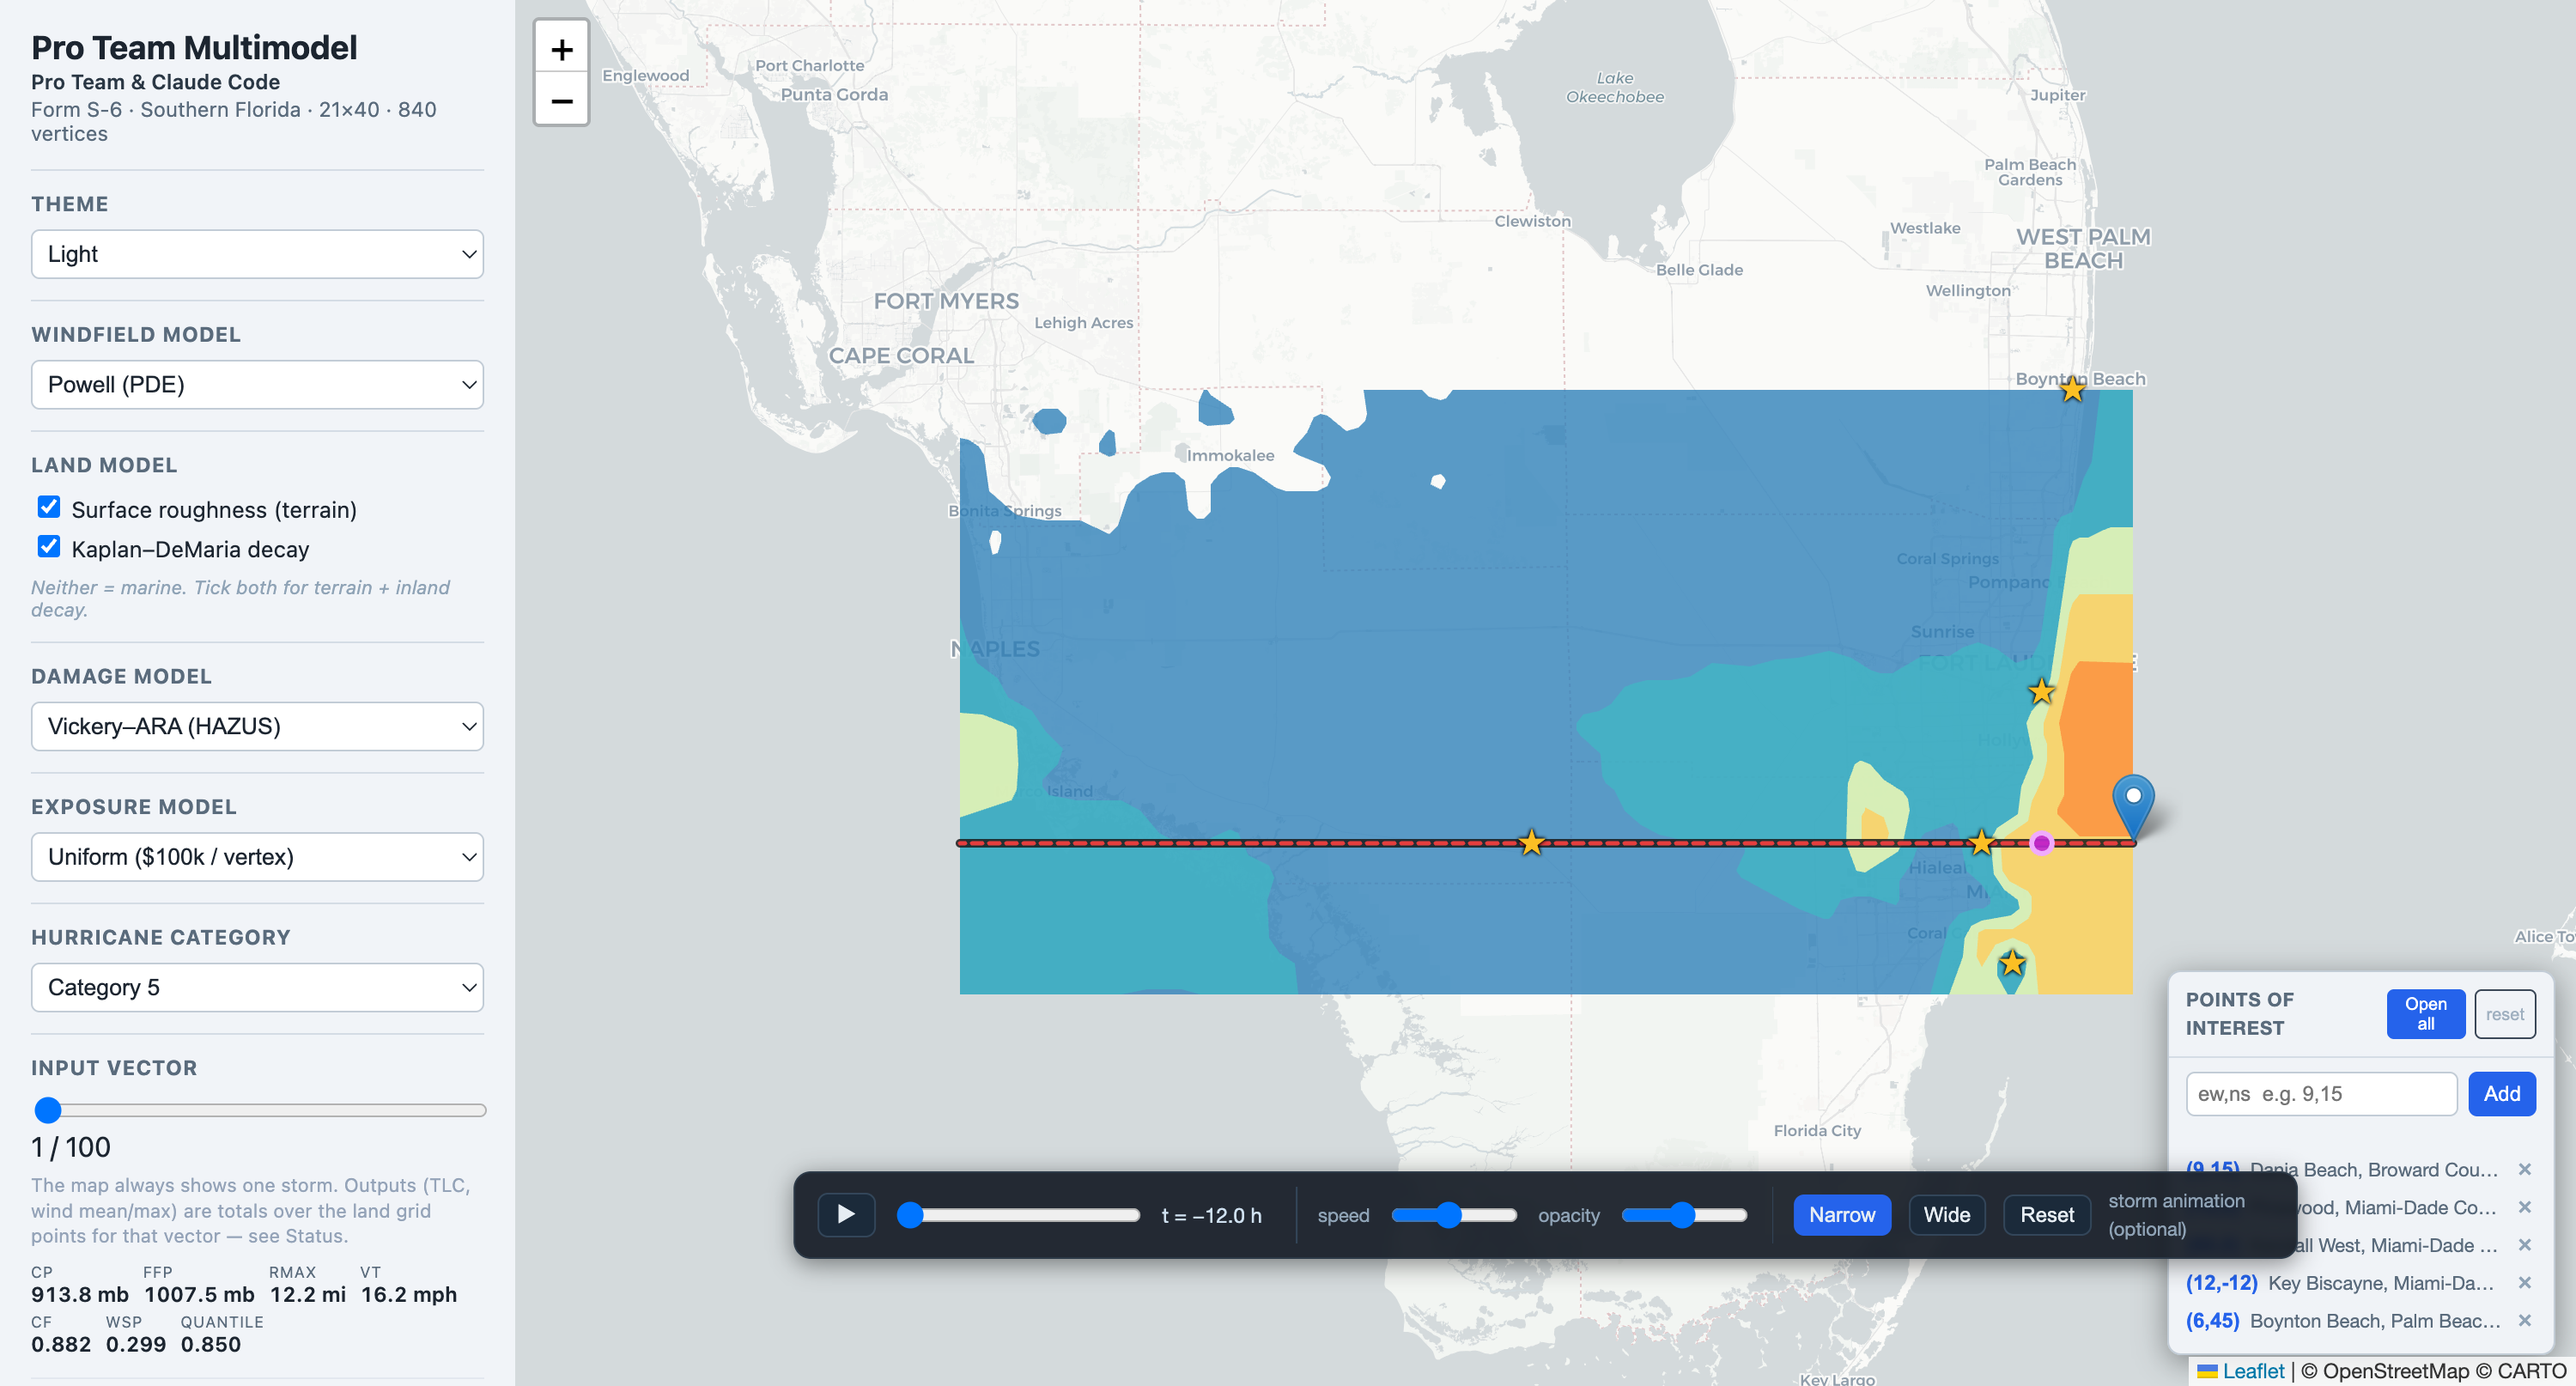
\includegraphics[width=0.55\textwidth]{powell_cat5_contour.png}
\caption{Powell peak-wind footprint (filled contours) for an intense example storm.
Strongest winds lie north of the track---correct for a westward-moving
Northern-Hemisphere cyclone, where translation adds to rotation on the north side.}
\label{fig:contour}
\end{figure}

\paragraph{Land effect: roughness and decay.} Two independent, combinable toggles model
the storm's interaction with land: \textbf{surface roughness} (a terrain-drag reduction
from NLCD land cover~\cite{nlcd} through published roughness tables~\cite{esdu,aersurface},
land-mean factor $\approx0.67$) and \textbf{Kaplan--DeMaria decay}~\cite{kaplan}
(inland weakening with a Gulf-recovery term). Both are on by default; turning both off
gives the marine field. For an intense storm the land-mean surface wind roughly halves
from marine to fully-land-adjusted.

\section{The storm population: a constrained, lumped design}
This is the conceptual heart of the current tool, and where it departs from the ROA's
category-stratified convention.

\paragraph{Six inputs.} Every storm is defined by central pressure CP, radius of maximum
wind $R_{\max}$, translation speed VT, the Holland shape parameter $B$, a
gradient-to-surface conversion factor CF, and far-field pressure FFP (pressure deficit
$\Delta p=\text{FFP}-\text{CP}$).

\paragraph{One population of 200, sampled with real dependence.} Rather than 100 storms
in each of Saffir--Simpson categories 1, 3, and 5 drawn independently, the app runs a
single \textbf{constrained lumped design of 200 storms} whose inputs honour the
dependence structure of the HURDAT2 best-track archive---most importantly the
central-pressure/radius coupling (CP\,$\sim R_{\max}$, correlation $r\approx0.43$) and a
radius-dependent shape parameter ($B$--$R_{\max}$, via Eq.~7 of Powell et
al.~\cite{powell}). Here $B$ is a \emph{direct} design input, not a quantile mapped
through a distribution. The legacy
3-category design is retained as an independent-inputs baseline and cross-check.

\paragraph{Why it matters.} Fixing a Saffir--Simpson category nearly fixes CP, so within
a category CP cannot express its influence---the classic framing structurally hides the
most important variable. Lumping the categories into one realistically-sampled population
lets CP vary over its full range, and it immediately becomes the leading driver
(see the Statistics section).

\section{Vulnerability: from wind to damage}
Damage is a \textbf{Mean Damage Ratio} (MDR), the fraction of a structure's value lost,
following the HAZUS/ARA wind-vulnerability methodology~\cite{hazus,vickery2006,araoir2024},
given as a smooth logistic function of peak wind: near zero below tropical-storm force,
rising steeply through the $100$--$150$\,mph range, and saturating toward $1$ for the
most extreme winds. The curve's midpoint, steepness, and cap are adjustable in the
viewer, so the vulnerability leg is itself a swappable model component. Because MDR is a
ratio, it is exposure-agnostic: it says what \emph{fraction} is lost, and the exposure
book (next section) says of \emph{how much}.

\section{Actuarial: exposure, loss cost, and financial metrics}

\paragraph{Loss cost.} At a land vertex the ground-up loss is
$\mathrm{LC}=\mathrm{MDR(wind)}\times\mathrm{exposure}$. The total loss a storm inflicts
is $\mathrm{TLC}(i)=\sum_{\text{land}}\mathrm{LC}$, and the headline ratio is
$\%\mathrm{TLC}(i)=\mathrm{TLC}(i)/(\text{total exposure})$.

\paragraph{Three exposure books.} Exposure is swappable: a \textbf{uniform}
\$100k/vertex reference (total \$68.2\,M), or realistic value surfaces from
\textbf{Census} (ACS home value) and \textbf{Tax Roll} (Florida cadastral) data. The
realistic books are extraordinarily concentrated---the densest Miami cell carries some
$1500\times$ the median, and the coastal Gini is $\approx0.84$---which changes loss
magnitudes by orders of magnitude and, crucially, changes which wind-field details
matter (a coastal wind shift moves the loss far more than an inland one).

\paragraph{Financial layer.} A financial panel adds the actuarial leg on top of
hazard $\times$ vulnerability: per-location deductible and limit, an exceedance-probability
(EP/OEP) curve of loss versus return period, and metrics---average annual loss (AAL),
50/100/250-year losses, and tail value-at-risk---driven by a single editable annual
landfall rate for the lumped population.

\section{Statistics: what drives the loss, and how sure are we}
\label{sec:stats}
The app reports three complementary sensitivity measures over the 200-storm population,
following the Commission's sensitivity/uncertainty demonstration~\cite{iman}.

\paragraph{SRC and EPR.} The \textbf{standardized regression coefficient} (SRC) gives
each input's first-order, linear influence (sign and magnitude); the \textbf{uncertainty}
measure EPR is reported as the variance share $\mathrm{SRC}_i^2$.

\paragraph{Shapley effects --- the primary, dependence-aware measure.} Because the
constrained inputs are correlated \emph{by construction}, the classical Sobol' variance
decomposition~\cite{sobol} (which assumes independent inputs) is not strictly valid. The
\textbf{Shapley effect}~\cite{owen2014,song2016} borrows the Shapley value from
cooperative game theory to apportion output variance among dependent inputs: the shares
are non-negative and sum exactly to one whatever the correlations. It is estimated with
a given-data nearest-neighbour estimator~\cite{broto2020}, and is the tool's primary
sensitivity method (Figure~\ref{fig:shapley}).

\paragraph{Sobol' as an independent-input cross-check.} The classical Sobol' indices are
still computed---sampling the marginals independently, with the Saltelli and Jansen
estimators~\cite{saltelli2010,jansen1999} on the emulator~\cite{francom}---as a reference. \textbf{The two
methods agree on the leaders}: on both peak wind and loss cost, \textbf{CP dominates}
(Shapley share $\approx0.45$--$0.51$) with $R_{\max}$ second ($\approx0.21$--$0.29$).
They diverge where dependence and the decay process bite hardest---on translation speed
VT (which the decay makes matter) and on $B$ (coupled to $R_{\max}$)---which is exactly
the behaviour a dependence-aware method is needed to get right. Agreement on the
headline is the reassurance of running two independent methods: \emph{we did the
irregular (Shapley) and the regular (Sobol') analysis, and they concur that central
pressure leads.}

\begin{figure}[H]
\centering
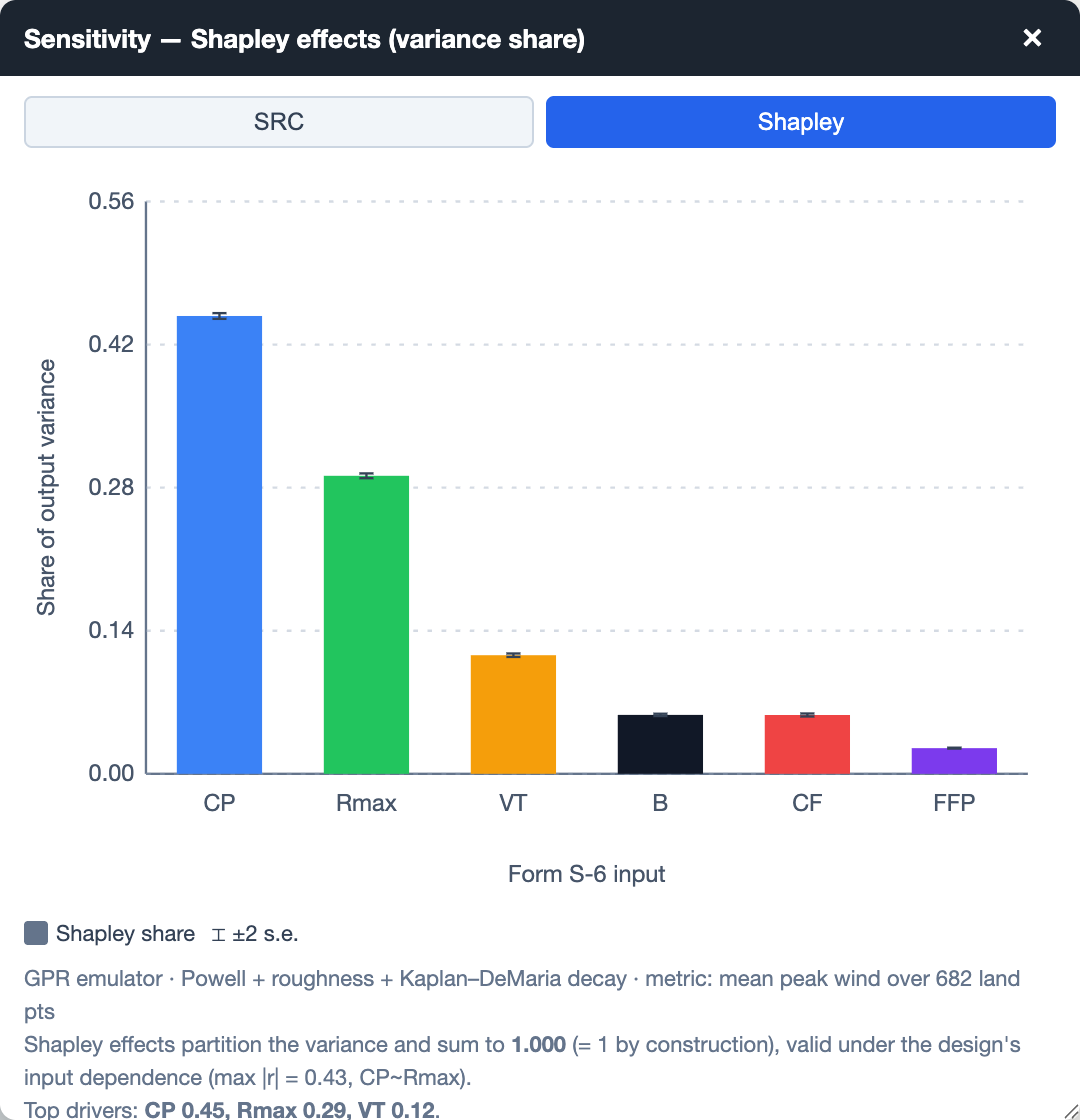
\includegraphics[width=0.6\textwidth]{analysis_shapley.png}
\caption{Shapley effects for peak wind on the constrained 200-storm population (shipped
default land configuration). CP dominates; $R_{\max}$ second; the six shares sum to one
by construction. This overturns the legacy per-category ranking, in which storm size or
profile shape led, because lumping frees CP to vary.}
\label{fig:shapley}
\end{figure}

\paragraph{Metamodels and the profiler.} The sensitivity measures run on a
\textbf{metamodel} (emulator) fit to the 200 runs---a second-order response surface, a
Gaussian-process regression, and a neural network, which agree and (because the
simulator is smooth) reach $R^2\approx1$; their value is diagnostic, not predictive. An
interactive \textbf{profiler} and \textbf{interaction matrix} let the user bend one
input at a time and see the response and the pairwise interactions directly. A hold-out
test on unseen storms confirms the emulator predicts to $R^2\ge0.998$.

\paragraph{Spatial sensitivity.} Sensitivity is also mapped \emph{per vertex}: the
dominant input varies across the grid, so a single grid-averaged ranking can mislead---an
off-track vertex is governed by storm size (does the wind reach it at all?) while the
domain average is governed by central pressure.

\section{Computer science: the implementation}
The deployed application is a \textbf{zero-backend static web page}
(HTML/CSS/JavaScript + Leaflet); it can be served from any static host. The pattern
throughout is \textbf{precompute-then-evaluate}: expensive physics (the Powell PDE, the
machine-learning emulators, the dynamic-storm animation frames) is computed offline in
Python and exported to compact JSON, and the browser only \emph{samples} it---so model
switches and analyses are instant and the site needs no server (Figure~\ref{fig:flow}).

\begin{figure}[H]
\centering
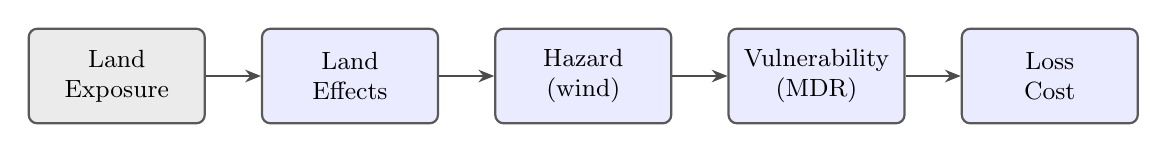
\begin{tikzpicture}[node distance=7mm]
  \node[dfsrc]                (exp)  {Land\\Exposure};
  \node[dfbox, right=of exp]  (land) {Land\\Effects};
  \node[dfbox, right=of land] (haz)  {Hazard\\(wind)};
  \node[dfbox, right=of haz]  (vul)  {Vulnerability\\(MDR)};
  \node[dfbox, right=of vul]  (loss) {Loss\\Cost};
  \draw[flow] (exp)--(land); \draw[flow] (land)--(haz);
  \draw[flow] (haz)--(vul);  \draw[flow] (vul)--(loss);
\end{tikzpicture}
\caption{The catastrophe-model chain the app implements. Exposure is conditioned by the
land effects, which shape the hazard; the hazard drives vulnerability; and vulnerability
against exposure yields loss costs. Each stage is a swappable model.}
\label{fig:flow}
\end{figure}

\paragraph{Interface at a glance.} The viewer offers model selection, an input-vector
slider over the 200 storms (no category selector---the population is unstratified), the
land-effect checkboxes, colour-by modes (wind, loss, land/water, dominant-sensitivity), a
points/contour display toggle, light/dark themes, hover read-outs, saved points of
interest with printable detail pages, an optional storm animation, and the analysis
panels (sensitivity, uncertainty, profiler, loss-cost CDF, and the financial EP curve).

\paragraph{Reproducibility.} The pipeline is public-domain and self-contained: a fresh
clone rebuilds every wind field, the damage curve, and every figure in the reports.
The Powell PDE solver and the wind-vulnerability tool are vendored in-repo; nothing the
pipeline needs lives outside the clone.

\section{The essentials, in five lines}
\begin{itemize}
\item \textbf{Meteorology:} three wind models (Powell/Holland/Willoughby) plus a
      time-dependent Powell, over the specified $840$-vertex South-Florida grid, with
      roughness and inland-decay land effects.
\item \textbf{Design:} one realistically-dependent population of 200 storms, not
      independent per-category draws.
\item \textbf{Statistics:} dependence-aware Shapley effects (primary) cross-checked by
      classical Sobol' (reference)---\textbf{central pressure is the dominant driver},
      $R_{\max}$ second.
\item \textbf{Loss:} MDR damage curve $\times$ a swappable exposure book (uniform,
      Census, or Tax Roll), with a full financial exceedance layer.
\item \textbf{Software:} a reproducible, zero-backend static web app---precompute in
      Python, evaluate in the browser.
\end{itemize}

\begin{thebibliography}{99}
\bibitem{fchlpm} Florida Commission on Hurricane Loss Projection Methodology (2025).
\emph{Report of Activities}. Standard S-3 and Form S-6.

\bibitem{iman} Iman, R.~L., Johnson, M.~E., and Schroeder, T.~A. (2001).
\emph{Professional Team Demonstration Uncertainty/Sensitivity Analysis}.
\url{https://fchlpm.sbafla.com/media/tepang2l/ua-sa-demo.pdf}

\bibitem{holland} Holland, G.~J. (1980). An analytic model of the wind and pressure
profiles in hurricanes. \emph{Monthly Weather Review}, 108, 1212--1218.

\bibitem{willoughby} Willoughby, H.~E., Darling, R.~W.~R., and Rahn, M.~E. (2006).
Parametric representation of the primary hurricane vortex. Part~II: A new family of
sectionally continuous profiles. \emph{Monthly Weather Review}, 134, 1102--1120.

\bibitem{powell} Powell, M.~D., Soukup, G., Cocke, S., Gulati, S.,
Morisseau-Leroy, N., Hamid, S., Dorst, N., and Axe, L. (2005). State of Florida
hurricane loss projection model: Atmospheric science component.
\emph{Journal of Wind Engineering and Industrial Aerodynamics}, 93(8), 651--674.

\bibitem{vickery} Vickery, P.~J., Wadhera, D., Powell, M.~D., and Chen, Y. (2009).
A hurricane boundary layer and wind field model for use in engineering applications.
\emph{Journal of Applied Meteorology and Climatology}, 48, 381--405.

\bibitem{smithvogl} Smith, R.~K., and Vogl, S. (2008). A simple model of the
hurricane boundary layer revisited. \emph{Quarterly Journal of the Royal
Meteorological Society}, 134, 337--351.

\bibitem{kaplan} Kaplan, J., and DeMaria, M. (1995). A simple empirical model for
predicting the decay of tropical cyclone winds after landfall.
\emph{Journal of Applied Meteorology}, 34, 2499--2512.

\bibitem{nlcd} Multi-Resolution Land Characteristics Consortium (2023).
\emph{NLCD 2021 Land Cover (CONUS)}. \url{https://www.mrlc.gov}.

\bibitem{esdu} ESDU (1985). \emph{Characteristics of atmospheric turbulence near the
ground. Part~II: Single point data for strong winds (neutral atmosphere)}. ESDU 85020.

\bibitem{aersurface} U.S. Environmental Protection Agency.
\emph{AERSURFACE User's Guide}, land-cover to surface-roughness ($z_0$) tables.

\bibitem{hazus} Federal Emergency Management Agency (2025). \emph{Hazus 7.0
Hurricane Model Technical Manual}. FEMA. (Wind vulnerability methodology developed
by Applied Research Associates.)

\bibitem{vickery2006} Vickery, P.~J., Lin, J., Skerlj, P.~F., Twisdale, L.~A.,
and Huang, K. (2006). HAZUS-MH hurricane model methodology. II: Damage and loss
estimation. \emph{Natural Hazards Review}, 7(2), 94--103.

\bibitem{araoir2024} Applied Research Associates, Inc. (2024). \emph{2024
Residential Wind-Loss Mitigation Study} (Report \#005480). Prepared for the
Florida Office of Insurance Regulation, Tallahassee, FL.

\bibitem{francom} Francom, D., and Nachtsheim, A. (2025). \emph{A Review and
Comparison of Different Sensitivity Analysis Techniques in Practice}. Los Alamos
National Laboratory. arXiv:2506.11471.

\bibitem{sobol} Sobol', I.~M. (2001). Global sensitivity indices for nonlinear
mathematical models and their Monte Carlo estimates. \emph{Mathematics and
Computers in Simulation}, 55, 271--280.

\bibitem{saltelli2010} Saltelli, A., Annoni, P., Azzini, I., Campolongo, F.,
Ratto, M., and Tarantola, S. (2010). Variance based sensitivity analysis of model
output. Design and estimator for the total sensitivity index. \emph{Computer
Physics Communications}, 181, 259--270.

\bibitem{jansen1999} Jansen, M.~J.~W. (1999). Analysis of variance designs for
model output. \emph{Computer Physics Communications}, 117, 35--43.

\bibitem{owen2014} Owen, A.~B. (2014). Sobol' indices and Shapley value.
\emph{SIAM/ASA Journal on Uncertainty Quantification}, 2, 245--251.

\bibitem{song2016} Song, E., Nelson, B.~L., and Staum, J. (2016). Shapley effects
for global sensitivity analysis: theory and computation. \emph{SIAM/ASA Journal on
Uncertainty Quantification}, 4, 1060--1083.

\bibitem{broto2020} Broto, B., Bachoc, F., and Depecker, M. (2020). Variance
reduction for estimation of Shapley effects and adaptation to unknown input
distribution. \emph{SIAM/ASA Journal on Uncertainty Quantification}, 8, 693--716.
\end{thebibliography}

\end{document}
